\subsection{Spændingsforstærker}
\label{effekt_spaendingsforstaerker}
Spændingsforstærkerens opgave er at give en så stor spændingsforstærkning som muligt. Til dette projekts spændingsforstærkning er der valgt en BC557B PNP-transistor koblet som en commonemitter. koblingen af spændingsforstærkeren er vist på figur \ref{spaendingsforstaerker_diagram}

\begin{figure}[h]
\centering
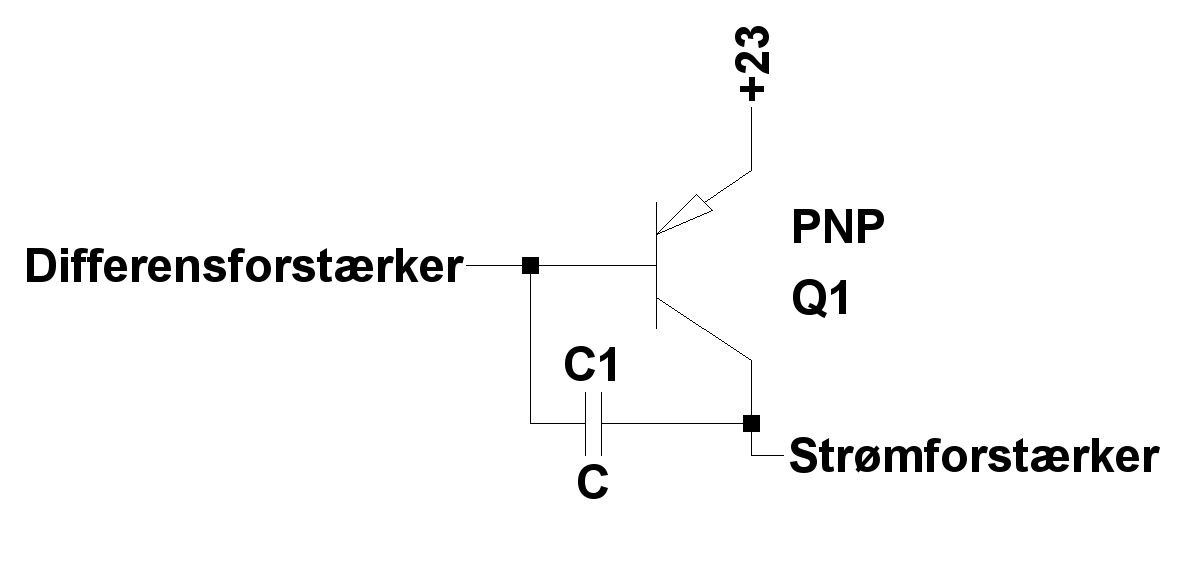
\includegraphics[width=\textwidth]{teknisk/effektforstaerker/spaendingsforstaerker_diagram.png}
\caption{Diagram over opbygningen af spændingsforstærkeren.}
\label{spaendingsforstaerker_diagram}
\end{figure}

Forstærkningen i en commonemitter kobling er bestemt ved ligning (\ref{equ:spaendingsforstaerker1}) 

\begin{equation}
\label{equ:spaendingsforstaerker1}
A_v = -g_m \cdot R'_L
\end{equation}

For at beregne $g_m$ bruges ligning \ref{equ:spaendingsforstaerker2} hvor $I_c$ er den collectorstrøm som konstantstrømsgeneratoren trækker, og $V_T$ er sat til at være konstant $26 mV$

\begin{equation}
\label{equ:spaendingsforstaerker2}
g_m = \frac{I_c}{V_T} = \frac{6 mA}{26 mV} = 230,8~mS
\end{equation}

Nu skal $R'_L$ beregnes. $R_L$ er defineret som den load spændingsforstærkeren ser. For at gøre det nemmere at beregne $R_L$ er der lavet nogle antagelse. Første antagelse er at $V_be$-Multiplieren når der kigges på AC kan betragtes som en kortslutning. Dette leder frem til den næste antagelse at konstantstrømsgeneratoren repræsentere en uendelig stor impedans. Det vil resultere i at den er meget større end de andre impedanser og derfor kan man ses bort fra den. Den sidste antagelse der er lavet er at kortslutningskredsløbet kan ses bort fra idet dette kredsløb ikke er aktuelt hvis systemet  kører som det skal. Med disse antagelser på plads kan $R_L$ beregnes ud fra parallelkoblingen mellem de to darlingtontransistorer.



For at kunne bregne $R_L$ er det nødvendigt at finde den impedans som darlingtontransistoren repræsentere. Darlingtontransistorerne der er valgt til projektet er opbygget som vist på figur \ref{darlington_diagram}. I databladet for darlingtontransistorerne \fixme{Kilde: BDX33B/BDX34B datablad}  er R1 angivet til typisk at være 10 k\ohm~og R2 til 150 \ohm.

\begin{figure}[h]
\centering
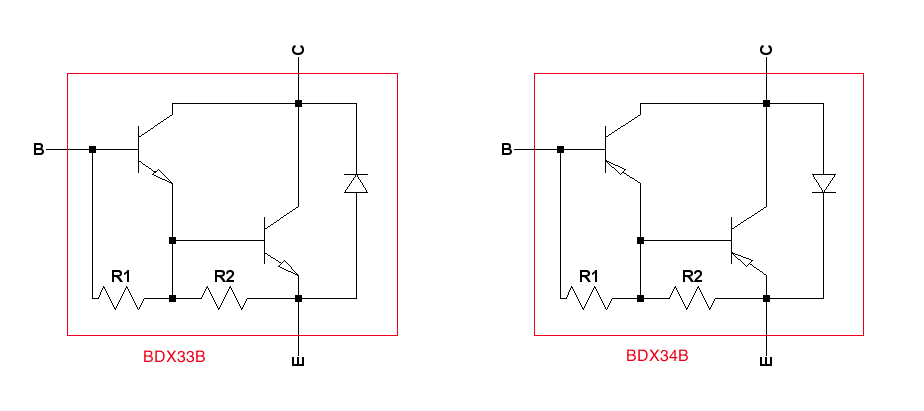
\includegraphics[width=\textwidth]{teknisk/effektforstaerker/darlingtontransistor_opbygning.png}
\caption{Diagram over opbygningen af darlingtontransistor BDX33B og BDX34B}
\label{darlington_diagram}
\end{figure}

For at gøre det nemmere at bestemme impedansen af darlingtontransistoren er det valgt at opfatte den som en enkelt supertransistor hvor $\beta = \beta_1 \cdot \beta_2$\fixme{Kilde: sedra/smidth sixth edition side 525}. Der er også valgt at se bort fra de indre modstande i darlingtontransistoren. Når dette er valgt kan darlingtontransistoren i dette tilfælde opfattes som en transistor i en commomcollector kobling. Dernæst kan der opstilles en hybrid--model for transistoren som er vist i figur \ref{hybridpimodel_darlington} 

\begin{figure}[h]
\centering
\includegraphics[width=\textwidth]{}
\caption{Hybrid- -model opstillet for supertransistor.}
\label{hybridpimodel_darlington}
\end{figure}



det valgt at se bort fra de indre modstande i darlingtontransistoren,